% \documentclass{thesis}
% \usepackage[margin=0.5in]{geometry}
% \documentclass[a4paper,10pt,draft]{thesis}
\usepackage{physics,amsmath, amsfonts, siunitx, amssymb, graphicx, slashed,subcaption}
\usepackage[utf8]{inputenc}
\usepackage[margin=1in]{geometry}
\usepackage[hidelinks]{hyperref}
\usepackage{xr-hyper}
\newcommand{\n}[1]{\nu_{#1}}
\newcommand{\na}{\nu_\alpha}
\newcommand{\nb}{\nu_\beta}
\newcommand{\ana}{\bar{\nu}_\alpha}
\newcommand{\an}[1]{\bar{\nu}_{\text{#1}}}
\newcommand{\anb}{\bar{\nu}_\beta}
\renewcommand{\a}{\alpha}
\renewcommand{\b}{\beta}
\newcommand{\ab}{\alpha\beta}


\renewcommand{\ne}{\nu_e}
\newcommand{\nm}{\nu_\mu}
\newcommand{\nt}{\nu_\tau}
\newcommand{\ns}{\nu_s}

\newcommand{\ane}{\bar{\nu}_e}
\newcommand{\anm}{\bar{\nu}_\mu}
\newcommand{\ant}{\bar{\nu}_\tau}
\newcommand{\ans}{\bar{\nu}_s}

\newcommand{\nee}{\nu_e \to \nu_e}
\newcommand{\nem}{\nu_e \to \nu_\mu}
\newcommand{\net}{\nu_e \to \nu_\tau}
\newcommand{\nes}{\nu_e \to \nu_s}

\newcommand{\nme}{\nu_\mu \to \nu_e}
\newcommand{\nmm}{\nu_\mu \to \nu_\mu}
\newcommand{\nmt}{\nu_\mu \to \nu_\tau}
\newcommand{\nms}{\nu_\mu \to \nu_s}



\newcommand{\Pee}{P_{e  e}}
\newcommand{\Pem}{P_{e  \mu}}
\newcommand{\Pet}{P_{e  \tau}}
\newcommand{\Pes}{P_{e  s}}

\newcommand{\Pme}{P_{\mu  e}}
\newcommand{\Pmm}{P_{\mu\mu}}
\newcommand{\Pmt}{P_{\mu  \tau}}
\newcommand{\Pms}{P_{\mu  s}}


\newcommand{\Pte}{P_{P_{\tau e}}}
\newcommand{\Ptm}{P_{\tau  \mu}}
\newcommand{\Ptt}{P_{\tau  \tau}}
\newcommand{\Pts}{P_{\mu  s}}

\newcommand{\Paeae}{P_{\bar{e}  \bar{e}}}
\newcommand{\Paeam}{P_{\bar{e}  \bar{\mu}}}
\newcommand{\Paeat}{P_{\bar{e}  \bar{\tau}}}
\newcommand{\Paeas}{P_{\bar{e}  \bar{s}}}

\newcommand{\Pamae}{P_{\bar{\mu}  \bar{e}}}
\newcommand{\Pamam}{P_{\bar{\mu}  \bar{\mu}}}
\newcommand{\Pamat}{P_{\bar{\mu}  \bar{\tau}}}
\newcommand{\Pamas}{P_{\bar{\mu}  \bar{s}}}


\newcommand{\Patae}{P_{\bar{\tau}  \bar{e}}}
\newcommand{\Patam}{P_{\bar{\tau}  \bar{\mu}}}
\newcommand{\Patat}{P_{\bar{\tau}  \bar{\tau}}}
\newcommand{\Patas}{P_{\bar{\mu}  \bar{s}}}

\renewcommand{\th}[1][]{%
  \theta\ifx\\#1\\\else_\text{#1}\fi
}
\newcommand{\thm}[1][]{%
  \theta^\text{M}\ifx\\#1\\\else_\text{#1}\fi
}
\renewcommand{\t}[1]{\text{{#1}}}
\newcommand{\avg}[1]{\left\langle {#1} \right \rangle}
\newcommand*{\dm}[1][]{%
  \Delta m^2\ifx\\#1\\\else_\text{#1}\fi
}
\newcommand{\zreco}{\cos{(\theta_z^{reco})}}
\newcommand{\ztrue}{\cos{(\theta_z^{true})}}
\newcommand{\z}{\cos{(\theta_z)}}
\newcommand{\Ereco}{E^{reco}}
\newcommand{\Etrue}{E^{true}}
\newcommand{\Aeff}{A^\text{eff}}
\newcommand{\emm}{\epsilon_{\mu\mu}}
\newcommand{\emt}{\epsilon_{\mu\tau}}
\newcommand{\eet}{\epsilon_{e\tau}}
\newcommand{\eem}{\epsilon_{e\mu}}
\newcommand{\ett}{\epsilon_{\tau\tau}}
\newcommand{\ep}{\epsilon^\prime}

% \begin{document}

\section{IceCube}\label{ch:ICmethod}
As the neutrinos have propagated the Earth, they arrive at the South Pole, where they interact with charged lepton in the ice. We now are interested in the effective area $\Aeff$, 
i.e.~the cross-section of the detector that the lepton is exposed to.
$\Aeff$ depends on several parameters, some of them being detector physical volume, $\Etrue$, $\ztrue$ and the neutrino cross-section. 
Fortunately, the binned $\Aeff$ is provided to us by the collaboration~\cite{ICaeff}.
The data file has the following form

\begin{table}[h]\label{table:aeff}
    \centering
    \begin{tabular}{lrrrrr}
        \hline \hline
        $\Etrue_{min}$ [\si{\GeV}] &     $\Etrue_{max}$ [\si{\GeV}]&   $\ztrue_{min}$ &   $\ztrue_{max}$ &     $\Aeff$ [\si{\metre\squared}] \\
        \hline
             251 &      316 &  -0.92 &  -0.91 &   0.0174 \\
          794300 &  1000000 &  -0.80 &  -0.79 &  69.3600 \\
            3981 &     5012 &  -0.78 &  -0.77 &   3.1490 \\
            1585 &     1995 &  -0.07 &  -0.06 &   0.4659 \\
            398 &      501 &  -0.73 &  -0.72 &   0.0555 \\
        \hline \hline
        \end{tabular}
    \caption{IceCube-86 effective area from~\cite{ICaeff}.}
\end{table}

Here, $\Aeff$ has been averaged over $\Aeff_\mu$ and $\Aeff_{\bar{\mu}}$.
Just as with the fluxes, we interpolate this in $\Etrue$, $\ztrue$ and show the result in Fig.~\ref{fig:aeff}
Since the IceCube array is slightly rectangular, the zenith angle affects the cross-sectional area of which the array the neutrinos are exposed to.
While the flux was almost flat in $\ztrue$, the introduction of the zenith dependent $\Aeff$ will make the result slightly more zenith dependent than 
the flux itself. Energy-wise, the situation here is completely reverse. Increasing with energy, the effective area of the detector
approaches its geometrical area of \SI{1e6}{\metre^2}, but is still only in the single digit range at \si{\TeV} energies.

\begin{figure}[t]\label{fig:aeff}
    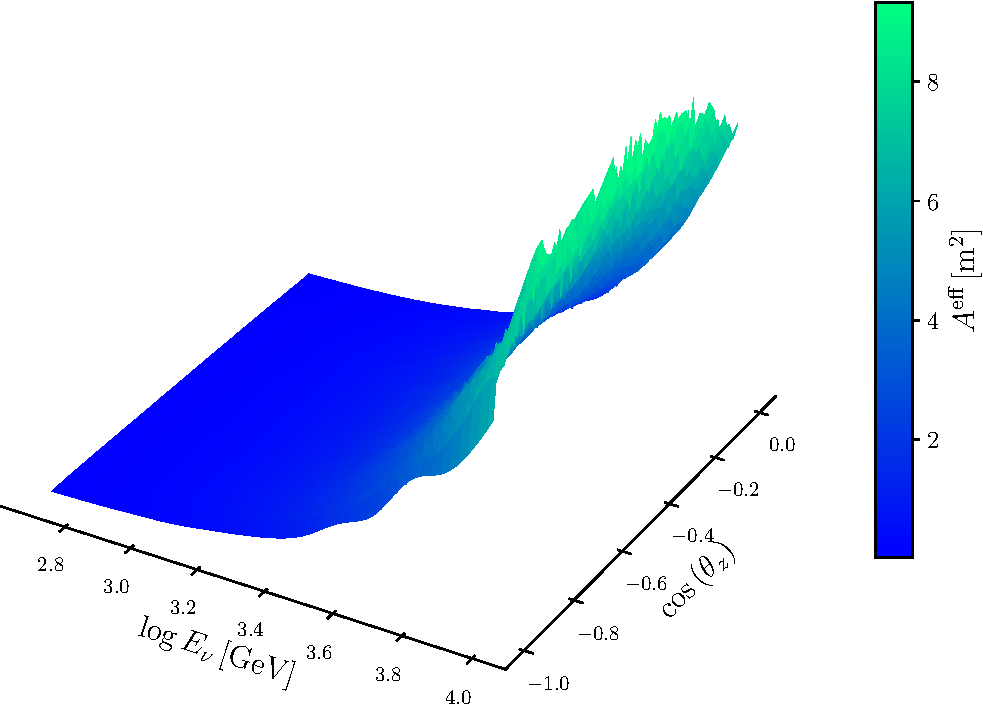
\includegraphics[width=0.7\textwidth]{figures/aeff.pdf}
    \caption{Interpolated IceCube effective area with data from~\cite{ICaeff}.}
\end{figure}

So now we have the physical quantities in the true parameters. But as we discussed, we need a way to translate this into the reconstructed parameters that the detector gives us. We will call the relationship between 
$\Ereco$ and $\Etrue$ the energy resolution function, and the relationshop between $\zreco$ and $\ztrue$ the zenith resolution function. We assume the relationship to follow a logarithmic Gaussian distribution, giving it the form 
\begin{align}\label{eq:gaussian}
    R(x^r, x^t) = \frac{1}{\sqrt{2\pi} \sigma_{x^r}x^r} \exp\left[-\frac{(\log x^r-\mu(x^t))^2}{2\sigma_{x^r}^2}\right]\,.
\end{align}
The parameters of the Gaussian are $\sigma_{x^r}(x^t)$ and $\mu(x^t)$, which are functions of the true parameters. By multiplying the Gaussian in Eq.~\ref{eq:gaussian}, we are reweighing the values by the 
probability density of that point. This process is also called \emph{smearing} because it effectively spreads out the data around a certain point. 

So how do we then obtain $\sigma_{x^r}(x^t)$ and $\mu(x^t)$ needed to construct the Gaussian? A Monte Carlo sample publically released by the 
collaboration has all the ingredients that we need~\cite{IC2016}. In Table.~\ref{table:IC_MC} we show a selection of the data.
The "pdg" column refers to the Monte Carlo particle classification, where 13 is the tag for $\nm$, while -13 refers
to an $\anm$. Here we note a crucial property of the IceCube dataset that will impact our analysis: the MC released by the collaboration
only includes simulated muon events.

\begin{table}[h]\label{table:IC_MC}
    \centering
    \begin{tabular}{lrrrrr}
        \hline \hline
        pdg &      $\Ereco$ [\si{\GeV}] &     $\zreco$ &       $\Etrue$ [\si{\GeV}] &     $\ztrue$ \\
        \hline
         13 &  1665 & -0.645884 &    592 & -0.653421 \\
         13 &   587 & -0.373241 &    342 & -0.424979 \\
        -13 &  1431 & -0.177786 &   1169 & -0.189949 \\
        -13 &   831 & -0.807226 &   1071 & -0.805559 \\
         13 &   988 & -0.370746 &   1861 & -0.367922 \\
         \hline \hline
  \end{tabular}
  \caption{A selection of the data found in~\ref{IC2016}}
\end{table}

First, we let $\zreco = \ztrue$ for all values. The angular resolution in IceCube for track-like events is less than $\SI{2}{\degree}$, making $\ztrue$ coincide with $\zreco$ for our study~\cite{IC2020}.
Thus, we only need to concern ourselves with the energy resolution.
In Fig.~\ref{fig:IC_MC_gpr}, we have plotted all event counts found in the MC file, over 8 million. However, this is too much data to process efficiently, with many outliers that ultimately don't weigh in 
that much in the final event count. To resolve this, we have opted to train a Gaussian process regressor on the dataset, from which we can extract the predicted mean and standard deviation for a point.
When doing this over $\Ereco$, we sample $\Etrue$ in the 99th percentile around the predicted mean. We then obtain the shaded band shown in Fig.~\ref{fig:IC_MC_gpr}. %TODO add plot with Etrue vs prob dens

The event rate for each bin reads
\begin{align}\label{eq:ICevents}
    N_{ij} &= T \sum_\beta\int_{(\cos{\theta_z^r})_i}^{(\cos{\theta_z^r})_{i+1}} \dd \cos{\theta^r_z} \int_{E^r_{j}}^{E^r_{j+1}} \dd E^r 
    \int_0^\pi R(\theta^r,\theta^t) \dd \cos{\theta^t} \int_0^\infty R(E^r,E^t) \phi_\beta^\text{det}  A^\text{eff}_\beta \dd E^t
    \,,
\end{align}
where $T$ is the live time of the detector. Now this expression handles the Gaussian smearing, but we are not provided systematic error sources, DOM efficiencies, and many more nuisance parameters. To correct this,
we will aim to come as close as possible to the IceCube Monte Carlo, and then normalize with it. That way, we know that our null hypotheses will align while we are free to form additional hypotheses with different 
physics parameters. The binned Monte Carlo events that IceCube used as their null hypothesis in the 2020 sterile analysis is shown in %TODO:MC vs myMC fig.


\begin{figure}[!tb]
    \begin{center}
       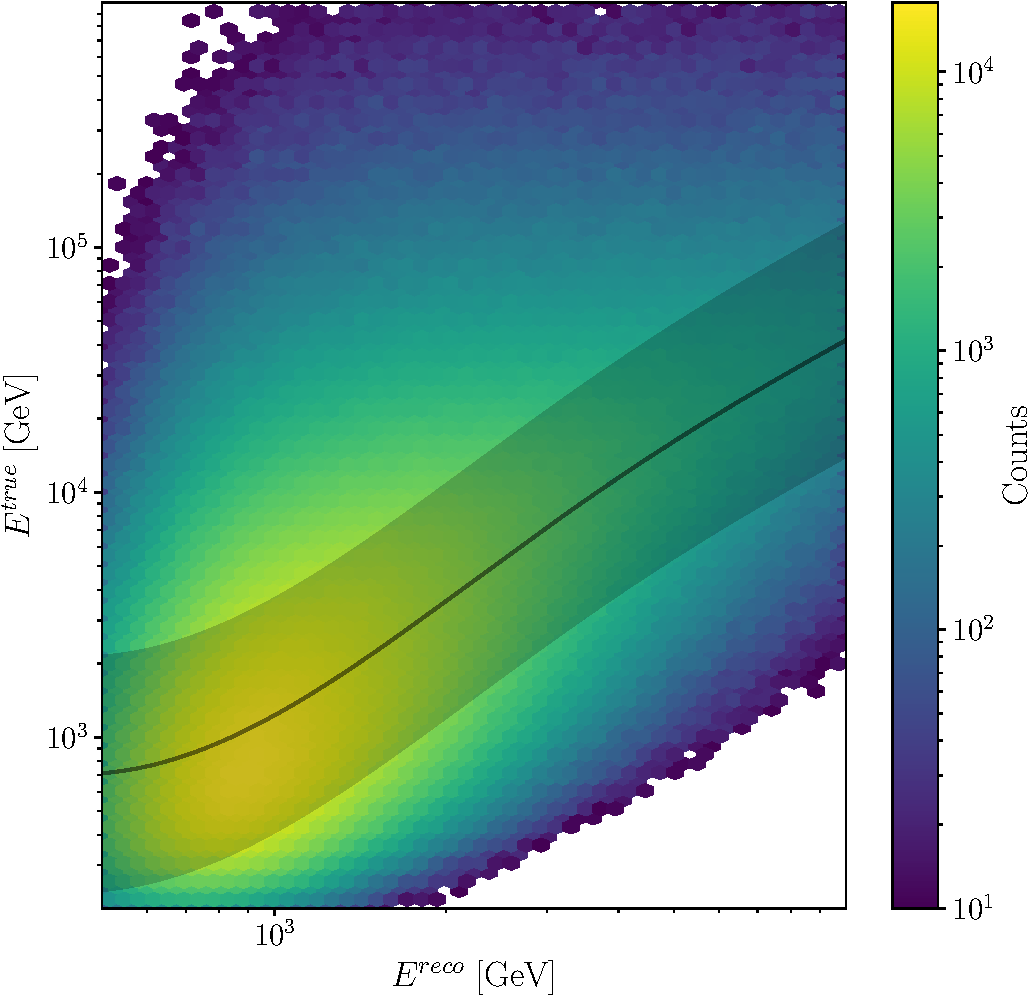
\includegraphics[width=0.4\linewidth]{figures/IC_MC_gpr.pdf}
    \end{center}
    \caption{Relationship between the true and reconstructed muon energy in the IceCube MC sample~\cite{IC2016}.
    Shaded area shows the $99.9$th percentile limits predicted by the regressor trained on this set.}\label{fig:IC_MC_gpr}
 \end{figure}

The latest available data collected and processed by the collaboration contains 305,735 muon track events, collected over eight years~\cite{IC2020}. 
%The data has 13 logarithmically spaced bins in $\Ereco \in \[500,9976\] \si{GeV}$, and 20 linear bins in $\zreco \in \[-1,0\]$. The data is shown in Fig.~\ref{fig:IC_data}.

\begin{figure}
    \centering
    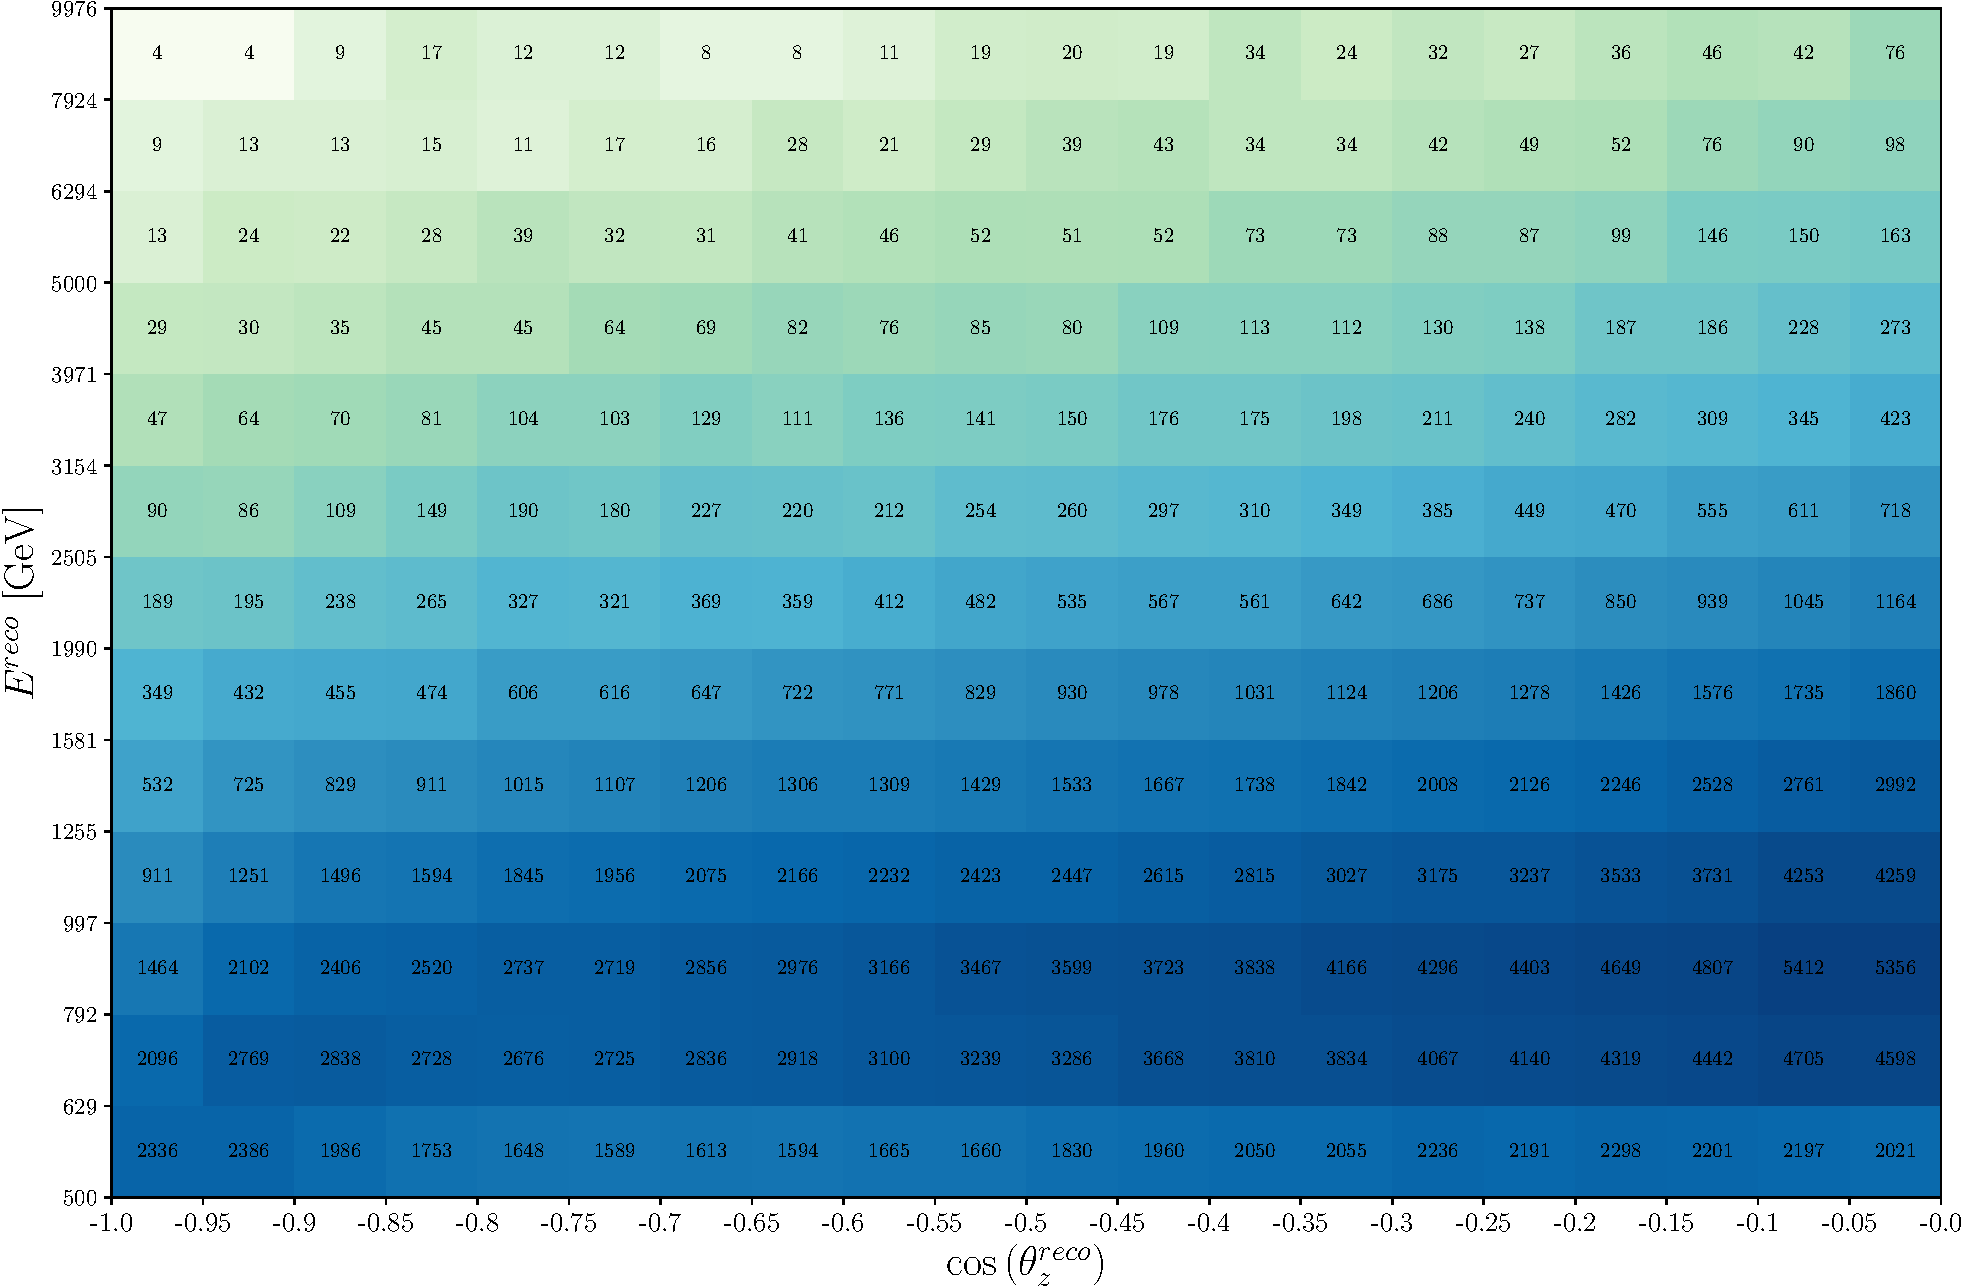
\includegraphics[width=0.8\linewidth]{figures/IC_data.pdf}
    \caption{IceCube track events from~\cite{IC2020}.}\label{fig:IC_data}
\end{figure}

\subsection*{Monte Carlo normalization}
Independent researchers outside of the IceCube collaboration will not be able to more percisely
simulate the detector. The IceCube Monte Carlo is a complex and proprietary machinery, so our goal in this 
section is to come as close as we can to their Monte Carlo simulations. After we are confident that 
our code displays the same overall features as the `offical', we normalize our results $N_{ij}^\text{sim}$ as 
\begin{align}\label{eq:MC_norm}
    N_{ij} = \frac{N_{ij}^\text{null}}{N_{ij}^\text{MC}} N_{ij}^\text{sim}\,.
\end{align}
For each bin $i,j$, we then obtain a correction factor which contains information that we are unable
to obtain or sufficiently incorporate. One example of such information is the systematic errors of the DOMs.
Recent IceCube data releases do not include such information. Since the systematic errors are affecting the 
event count on a bin-by-bin basis, they can in theory drastically modify the binned results. Another example of
an error source what will be remedied by this method is the flux. We are using a fairly simple model of the atmospheric 
flux that excludes atmospheric prompt and astrophysical fluxes. The IceCube collaboration use several different flux models which are initialized 
by a parametrization of the cosmic ray flux.\footnote{Included in the cosmic ray models are e.g. the pion to kaon 
ratio, which are often used as a nuisance parameter. By not being able to include this in our error analysis, our method will 
be limited to only consider the overall flux normalization, rather than the components that produce the flux in the first place.}

In Fig.~\ref{fig:IC_MC_norm}, we present the Icecube Monte Carlo obtained from their 2020 sterile analysis~\cite{IC2020}, along
with our null hypothesis times a constant factor.  We deemed these shapes to be satisfactory, thus allowing us to multiply Eq.~\ref{eq:ICevents} by the 
correction factors of Eq.~\ref{eq:MC_norm}. We now arrive to our final event count
\begin{align}\label{eq:Nth}
    N_{ij} &= \frac{N_{ij}^\text{null}}{N_{ij}^\text{MC}} T \sum_\beta \int_{(\cos{\theta_z^r})_i}^{(\cos{\theta_z^r})_{i+1}} \dd \cos{\theta^r_z} \int_{E^r_{j}}^{E^r_{j+1}} \dd E^r 
    \int_{E^t_{min}}^{E^t_{max}} R(E^r,E^t) \phi_\beta^\text{det}  A^\text{eff}_\beta\, \dd E^t
    \,,
\end{align}
with $E^t_{min}$, $E^t_{max}$, and $R(E^r,E^t)$ taken from the Gaussian process regressor.
\begin{figure}
    \centering
    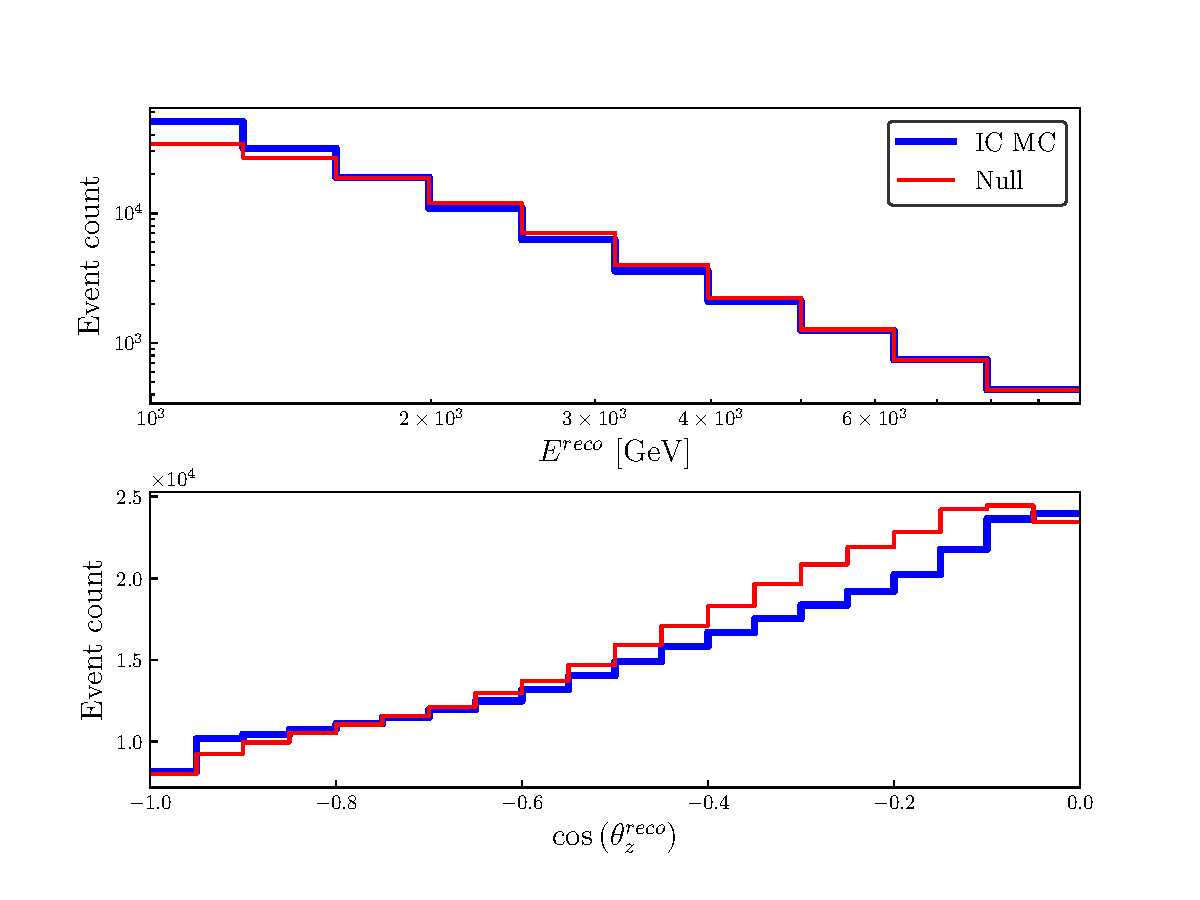
\includegraphics[width=0.8\linewidth]{figures/IC_MC_norm.pdf}
    \caption{IceCube Monte Carlo, binned in $\Ereco$ and $\zreco$. We compare this with our simulations shown as `Null' in the plots.}\label{fig:IC_MC_norm}
\end{figure} 
Thus, we are now able to sufficiently approximate the IceCube Monte Carlo, which makes us able to run simulations based on different physics scenarios.
% \newpage
% \bibliographystyle{nature}
% \bibliography{ref.bib}
% \end{document}